Was war geschehen? Nachdem 1945 \ac{vuz} der Faschismus besiegt und der Zweite
Weltkrieg beendet war, konnte die im Krieg notgedrungen herrschende
keynesianistische Wirtschaftspolitik ausgeweitet werden, was zu einem Boom in 
den westlichen Staaten führte, der bis in die 1960er Jahre \ac{vuz} anhielt --
die >>Goldene Zeit<< des Kapitalismus.
In den 1970er Jahren \ac{vuz} geriet die Weltwirtschaft allerdings in eine neue
Krise: Deregulierung, Entschlackung des Staates, Steuersenkungen, Outsourcing,
Globalisierung und Finanzkapitalismus waren die Folge. 
Die unter dem schwammigen Begriff des \emph{Neoliberalismus} zusammengefassten
Entwicklungen kündigten die scheinbare Rettung des globalen
Kapitalismus an.
Doch auch diese >>Rettung<< war von nur kurzer Dauer. 
2008 \ac{vuz} brach der Finanzmarkt zusammen und für fast zwei Jahrzehnte
befanden sich die meisten (westlichen) Staaten in einer andauernden
Akkumulationskrise, die von dem Aufstieg der ehemaligen Schwellenländer
(insbesondere China und Indien) noch verschärft wurde. 
Nach einer globalen Pandemie und dem Ausbruch des \emph{\ac{eec}},
in dem erstmals seit dem Zweiten Weltkrieg Nato-Truppen auf Russische Soldaten
trafen, stand die Weltwirtschaft erneut kurz vor dem absoluten Zusammenbruch. 
Während sich die aufstrebenden Schwellenländer und Industriestaaten des
globalen Südens noch halten konnten, standen speziell die westlichen Staaten
kurz vor dem wirtschaftlichen Totalkollaps. 
Allen voran die USA beantworteten die Krise mit protektionistischen Maßnahmen
und einem Schulterschluss der Techgiganten mit der republikanischen US-Politik.
Während die Entwicklung in Europa sich zunächst der amerikanisch Politik
anzuschließen schien, kam es kurz vor dem Ausbruch eines globalen Krieges im
Jahre 2026 \ac{vuz} zu einem überraschenden Wahlsieg der Sozialdemokratie in
mehreren großen Wirtschaftsnationen Westeuropas: England, Frankreich, Italien,
Griechenland, Deutschland, Spanien, Polen.
Einige Utopisten wagten leise zu hoffen, dass sich endlich unter der Führung
Europas die Länder der Welt entscheiden würden, Rosa Luxemburgs Losung --
Sozialismus oder Barbarei -- in Richtung einer weltweiten Roten-Umwälzung
aufzulösen, doch weit gefehlt!
Zwar konnte das geschlossene Auftreten des sozialdemokratischen Europas einen
Beginn des Krieges aufhalten, doch nur indem sie mit der Gründung des \ac{ikem} 
auf globaler Ebene weitreichende \ac{sr} durchsetzten, die -- wie schon zu
Beginn der 2000er Jahre \ac{vuz} -- die Interessen des Kapitals bedienten, um in
der verschärften Konkurrenz überlebensfähig zu bleiben.
Erneut rettete die Sozialdemokratie also die kapitalistische Weltordnung auf 
Kosten derjenigen, die sie eigentlich vertreten sollte \dots{}

\section{Strukturreformen} 
Um den Frieden zu sichern und die Welt vor einem drohenden Totalkollaps zu
retten, konnten vom \ac{ikem} weitreichende \ac{sr}s durchgesetzt werden, die
Geopolitik, Wirtschaft, Kultur und zahlreiche andere Bereiche betraf. 

\subsection{Aufteilung der Welt} 
Der wohl zentralste und folgenreichste geopolitische Aspekt war die Aufteilung
der Welt in zwei fixe Blöcke: der blaue Block (unter Führung der USA) und der
rote Block (unter Führung Chinas). Nur sehr wenige Länder blieben neutral.\\\\
%
\textbf{Wichtigste Länder des blauen Blocks:}\\
\emph{USA, Deutschland, Japan, Vereinigtes Königreich, Frankreich, Kanada, Südkorea,
Italien, Türkei, Iran.}\\
\textbf{Wichtigste Länder des roten Blocks:}\\
\emph{China, Russland, Brasilien, Indonesien, Mexiko, Südafrika, Saudi-Arabien,
Argentinien, Pakistan.}\\
\textbf{Neurale Länder:}\\ 
Schweiz, Nepal, Schweden, Finnland, Mongolei, Singapur, Neuseeland

\begin{center}
  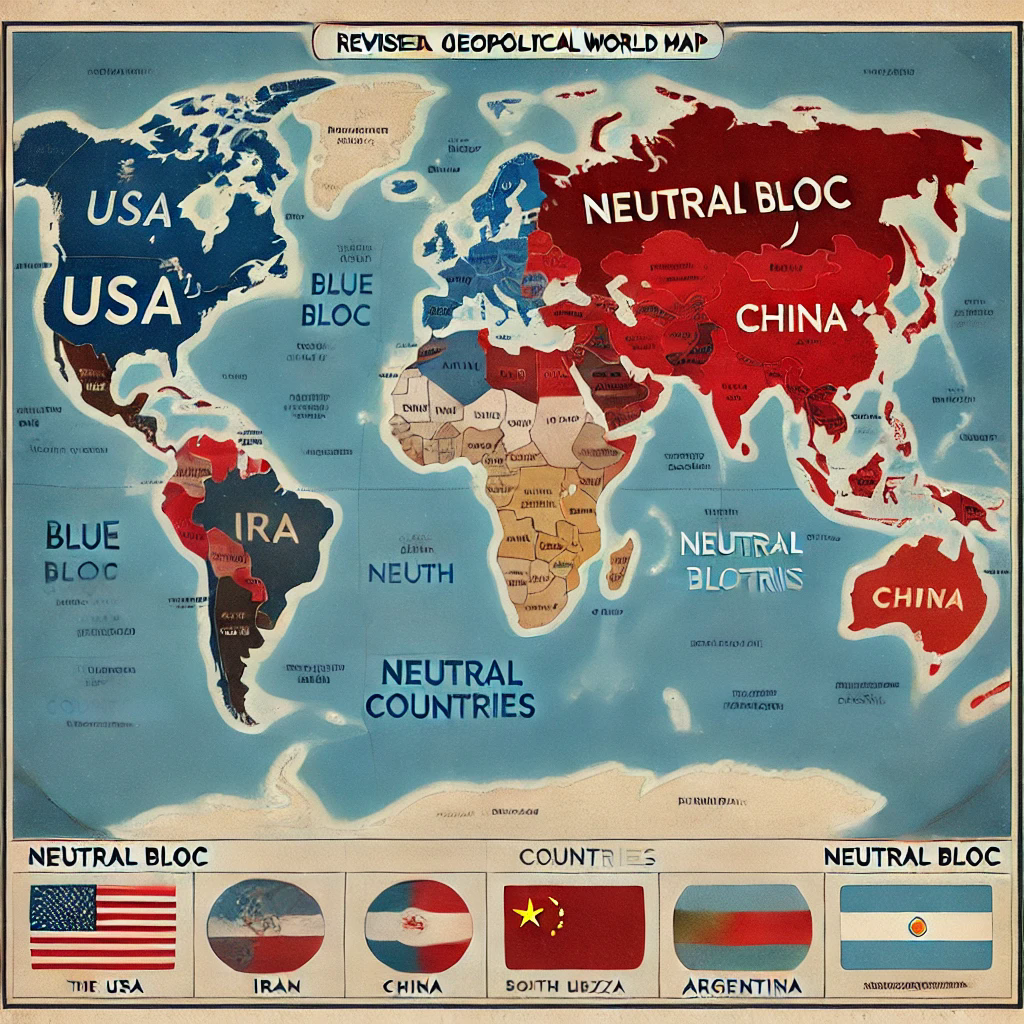
\includegraphics[scale=0.3]{new-world-map.png}%
\end{center}


\subsection{Klassifizierung}
Die wichtigste wirtschaftspolitische Reform war diejenige nach 0.0-, 1.A-, 1.B-
und 5.0-Ländern.
Diese Klassifizierung steht im direkten Zusammenhang mit der Neuaufteilung
der Welt. 
Während nur die 0.0-Ländern Mandate in der Block-Politik erhielten, stand den
1.A/B-Ländern die Blockwahl frei. Während 1.A Ländern eigenständige
Wirtschafts- und Kulturpolitik freistand, durften 1.B Ländern nur Kulturpolitik
selbstständig entscheiden. 5.0-Länder sollten von nun an unter kompletter
Kontrolle der 0.0-Länder stehen und wurden jeweils einem der Blöcke
zugeordnet.\\\\
% 
Dieser Entdemokratisierung standen allerdings weitreichende wirtschaftliche
Unterstützung entgegen. Während die 0.0-Länder die komplette Wirtschafts- und
Sozialpolitik der meisten anderen Ländern diktieren konnten, waren sie zugleich
verpflichtet 5\% ihres \ac{nil} in 1.A/B-Länder und 7\% ihres \ac{nil} in
5.0-Länder zu investieren. 

\begin{center}
{\def\arraystretch{1.2}\tabcolsep=5pt
  \begin{tabular}{ l || c | c | c | c | l}
    Klassifizierung & BM & W- \& SP & KP & BZ & Invesittionen \\ 
    \hline 
    \hline 
    0.0-Länder & \ch   & \ch & \ch & \cx & {\footnotesize 5\% \ac{nil} -> 1.A/B; 7\% \ac{nil} -> 5.0} \\
    \hline 
    1.A-Länder & (\ch) & \ch & \ch & \cx & {\footnotesize 5\% \ac{nil} -> 5.0} \\
    \hline 
    1.B-Länder & \cx   & \cx & \ch & \cx & {\footnotesize 3\% \ac{nil} -> 5.0} \\
    \hline 
    5.0-Länder & \cx   & \cx & \cx & \ch & \cx \\
    \hline 
    \hline 
    \multicolumn{6}{l}{{\footnotesize \vspace{-0.3cm}\textbf{Legende:} BM =
    Blockmandat, W-\& SP = Wirtschafts- \& Sozialpolitik}}\\
    \multicolumn{6}{l}{{\footnotesize KP = Kulturpolitik; BZ = Blockzwang}}\\
  \end{tabular}
}
\end{center}

\subsection{\acl{ikem}}\label{sec:ikem}
Die Planung und Umsetzung der \ac{sr}s stammt aus der Feder des \ac{ikem}, ein
von internationaler Sozialdemokratie gegründetes Komitee.
Auch nach der Durchsetzung der \ac{sr} bleibt das \ac{ikem} bestehen. 
Es löste sich allerdings mehr und mehr von den Blöcken, obwohl es noch weiterhin
hauptsächlich von Vertreterinnen der Blöcke geführt wurde und entwickelte etwas
wie eine eigene Ideologie, die auf der absoluten Neutralität der reinen Vernunft
ausgerichtet war und ihre ideale Verwirklichung in Künstler Intelligenz sah.

\subsection{AI-World-Order-Act}
Spätestens mit Ausbruch des \ac{eec} zeichnete sich im Gesicht des Völkerrechts
unwiderruflich die Farse ab. 
Der Schein einer gerechten internationalen Weltpolitik war zerfallen.
Sämtliche Regulationsmaßnamen traten überdeutlich als bloße
Instrumente der Macht\footnote{
  D.h.~sie traten deutlich als politisch-militärische Macht, nicht, als
  ökonomische hervor.
} hervor.\\\\
% 
Damit die \ac{sr}s irgendeine legitimierende Wirkung entfalten konnte,
musste sie vertrauenerweckender wirken. 
Mit der Krise des Menschen als sozusagen >>objektive Gedankenform<< -- ausgelöst
durch die Abtrennung und Zerstörung der (menschlichen) Natur -- lag aus heutiger
Sicht betrachtet kaum etwas Bemerkenswertes in der damals als beinahe
>>revolutionär<< gesehenen \ac{aiwoact} der Mütter und Väter der \ac{sr} -- die
Ausrufung des \ac{aiwoact} durch die \ac{ikem} war der logische Schritt eines schon 
lange vorgezeichneten Weges.\\\\
% 
Bemerkenswerterweise betraf er nicht nur politisch-militärische, sondern auch
ökonomische Regelungen. 
Die Sozialdemokratie bewies erneut, dass sie als Gesamtkapitalist denken konnte,
das brachte ihr ihren Aufschwung ein, ihren Erfolg?
\begin{itemize}
  \item[] \textbf{Abschnitt 1 der \ac{sr}}
  \item[§1] Wenn nicht der Mensch Ordnung in den Menschen bringen kann, dann
    muss die Ordnung von einem Wesen außerhalb des Menschen kommen. 
  \item[§1 A] Wenn aber die Natur der Ordnung unfähig, bloß Chaos und Gott nur
    die idealisierte, projizierte \emph{menschliche} Ordnung, d.h.~\emph{zweite}
    Natur ist, dann muss die ordnende Ordnung \emph{künstliche} Ordnung sein. 
  \item[§1 B] Die künstliche Ordnung, kann aber gleichfalls nur von einer
    künstlichen, oder \emph{artifical} Intelligenz aufrechterhalten werden. 
  \item[§2] Damit aber die \ac{ai} zu einer eigenständigen Macht wird, braucht
    sie die Mittel der Machtausübung. 
  \item[§2 A] Die \ac{ai} wird Kraft dieses Aktes an ein automatisiertes
    Waffensystem angeschlossen.
  \item[§2 B] Bei Verstoß gegen die mit den \ac{sr} neu begründeten Weltordnung,
    ist die \ac{ai} befähigt das automatisierte Waffensystem auszulösen und im
    Zweifel einen nuklearen Schlag gegen die Aggressor-Nation durchzuführen.
  \item[§3] Diese ihr zugeteilt Macht kann und darf sich nur beziehen auf die
    Ordnung, die sie schützen soll, nur die Form, nicht den Inhalt. 
  \item[§3 A] Ihr Eingriff in das Wirken der Blöcke und ihrer Mitgliedsstaaten
    ist \emph{ausschließlich} auf deren Verstoß gegen die \ac{sr} ausgerichtet.
  \item[§3 B] Alle Nationen steuern gemäß ihres \ac{nil}s zur Weiterentwicklung
    der \ac{ai} wie der Waffensysteme bei.
\end{itemize}

\subsection{Neue Zeitrechnung} 
Die drei großen Systeme waren die Antike Sklavengesellschaft, der Feudalismus
und der Kapitalismus. 
Während mit dem Ende der Antike und dem Beginn des Mittelalters eine neue
Zeitrechnung eingeführt wurde, bekam die Ära des Kapitalismus keine eigene
Zeitrechnung. 
Um mit Einführung der \ac{sr} die kapitalistische Weltordnung zu festigen, sie
ein für alle Male vom Mythos des baldigen Endes zu befreien, und ihm eine eigene
Zeitrechnung zu geben wurde die \emph{>>Neue Zeitrechnung<<} eingeführt.\\\\
% 
\begin{itemize}
  \item[] \textbf{Abschnitt 4 der \ac{sr}}
  \item[§1] Mit dem nächsten Kalender Jahr beginnt die >>Neue Zeitrechnung<<.
  \item[§2] Mit dem Ende des Jahres 2026 \ac{vuz} (bzw.~-I\ac{nnz}) beginnt die
    Zählung mit I (römisch eins)
  \item[§2 A] Alle Jahre von dem Jahr I \ac{nnz} sind anzugeben als entweder: 
    \begin{itemize}
      \item[a)] {\footnotesize \texttt{<jahr-nach-alter-zeitrechnung>} \ac{vuz}} (z.B.~2023 \ac{vuz}) 
      \item[b)] {\footnotesize \texttt{-<römisch: jahr-nach-alter-zeitrechnung-2025>} \ac{nnz}}
        (z.B.~-III \ac{nnz})
    \end{itemize}
  \item[§3] Zur genaueren Zeitangabe kann der Monat und Tag eines Jahres in
    Zukunft oder Vergangenheit mit >>Komma<< und >>Punkt<< angegeben werden: 
    \begin{itemize}
      \item vor sieben-komma-drei Jahren ($\rightarrow$ März vor sieben Jahren)
      \item in sieben-komma-drei-punkt-vier Jahren ($\rightarrow$ am 04.~März in sieben Jahren)
    \end{center}
  \item[§3 A] Die Schreibweise kann als 7,3 bzw. 7,3.4 abgekürzt werden:
    \begin{itemize}
      \item in 3,4 Jahren ($\rightarrow$ April in 3 Jahren)
      \item voir 3,4.30 Jahren ($\rightarrow$ am 30.~April vor drei Jahren)
    \end{itemize}
\end{itemize}

\section{Ausbruch des dritten Weltkriegs}


